% Slide 19: What is Data Mining?
\begin{frame}{داده‌کاوی چیست؟}
\begin{columns}[T,onlytextwidth]
\begin{column}{0.65\textwidth}
\begin{itemize}
  \item \textbf{جمع‌آوری پیوسته و انبوه داده‌ها:}
  \begin{itemize}
    \item داده‌های عظیمی درباره تمامی ابعاد زندگی و حرفه ما ثبت می‌شوند
    \item این داده‌ها حاوی الگوها و روندهای بسیار ارزشمند و پنهانی هستند
  \end{itemize}
  \vspace{0.2cm}
  \item \textbf{داده‌کاوی} (\lr{Data Mining}) به ما کمک می‌کند تا
  \begin{enumerate}
    \item این الگوهای پنهان را کشف کنیم (\lr{Discover patterns})
    \item از آن‌ها برای تصمیم‌گیری هوشمندانه در تمام ارکان جامعه بهره ببریم:
    \begin{itemize}
      \item کسب‌وکار، اقتصاد و صنایع تولیدی
      \item علوم بنیادین، محاسباتی و مهندسی
      \item پزشکی، سلامت و زیست‌فناوری
      \item حاکمیت و تصمیم‌گیری‌های دولتی
      \item تصمیم‌گیری‌های روزمره شهروندان
    \end{itemize}
  \end{enumerate}
\end{itemize}
\end{column}
\begin{column}{0.32\textwidth}
\begin{center}
  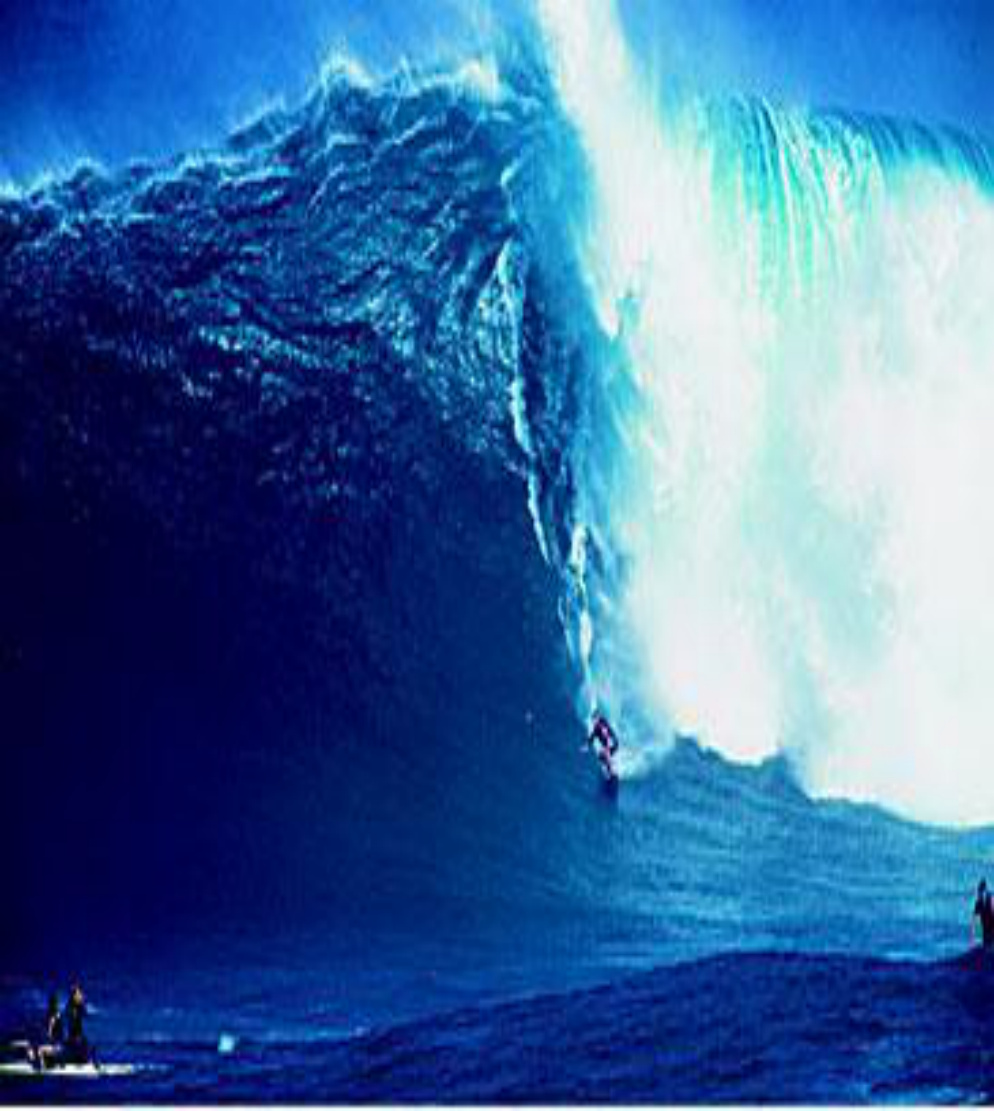
\includegraphics[width=\textwidth,height=4cm,keepaspectratio]{images/img_p19_2_110.jpeg}\\[0.1cm]
  {\fontsize{6.5}{8}\selectfont\color{subgray}موج سهمگین داده‌ها در عصر اطلاعات}
\end{center}
\end{column}
\end{columns}
\end{frame}

% Slide 20: Drowning in Data - CERN
\begin{frame}{ما در داده‌ها غرق شده‌ایم...}
\framesubtitle{مرکز پژوهش‌های هسته‌ای اروپا (\lr{CERN})}
\begin{columns}[T,onlytextwidth]
\begin{column}{0.6\textwidth}
\begin{itemize}
  \item \textbf{برخورددهنده بزرگ هادرونی} (\lr{LHC})
  \begin{itemize}
    \item تولید هفتگی \lr{45} پتابایت داده جدید (\lr{February 2024})
    \item آرشیو بیش از \lr{820} پتابایت داده روی نوارهای مغناطیسی
    \item دسترسی به بیش از \lr{1005} پتابایت فضای دیسک پرسرعت (\lr{August 2024})
  \end{itemize}
  \vspace{0.3cm}
  \item \textbf{هدف اصلی داده‌کاوی:}
  \begin{itemize}
    \item کشف ذرات، الگوهای نادر و پدیده‌های ناشناخته فیزیکی در آزمایش‌ها
  \end{itemize}
\end{itemize}
\end{column}
\begin{column}{0.37\textwidth}
\begin{center}
  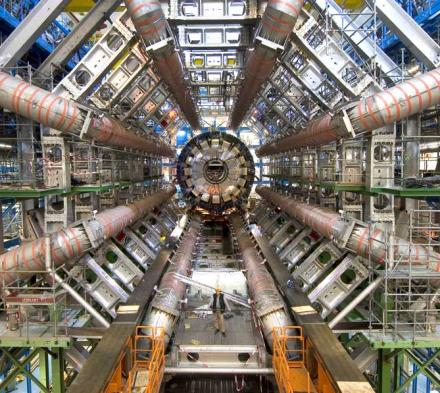
\includegraphics[width=0.85\textwidth,height=2cm,keepaspectratio]{images/img_p20_1_122.jpeg}\\[0.15cm]
  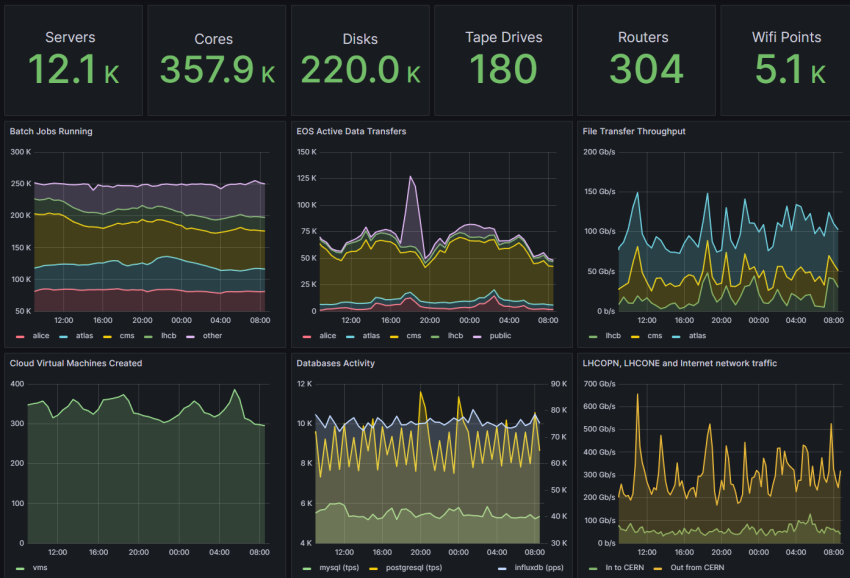
\includegraphics[width=0.95\textwidth,height=2.2cm,keepaspectratio]{images/img_p20_2_123.png}
\end{center}
\end{column}
\end{columns}
\end{frame}

% Slide 21: Drowning in Data - Facebook
\begin{frame}{ما در داده‌ها غرق شده‌ایم...}
\framesubtitle{شبکه‌های اجتماعی و کلان‌داده (\lr{Facebook})}
\begin{columns}[T,onlytextwidth]
\begin{column}{0.55\textwidth}
\begin{itemize}
  \item \textbf{حجم اطلاعات فیس‌بوک:}
  \begin{itemize}
    \item تولید روزانه \lr{4} پتابایت داده خام جدید توسط کاربران
    \item انباشت بیش از \lr{300} پتابایت در انبار داده فیس‌بوک (\lr{Data Warehouse})
  \end{itemize}
  \vspace{0.3cm}
  \item \textbf{پیش‌بینی و تحلیل الگوها:}
  \begin{itemize}
    \item پیش‌بینی علایق، رفتار و کنش‌های بیش از \lr{1} میلیارد کاربر در سراسر جهان
  \end{itemize}
\end{itemize}
\end{column}
\begin{column}{0.42\textwidth}
\begin{center}
  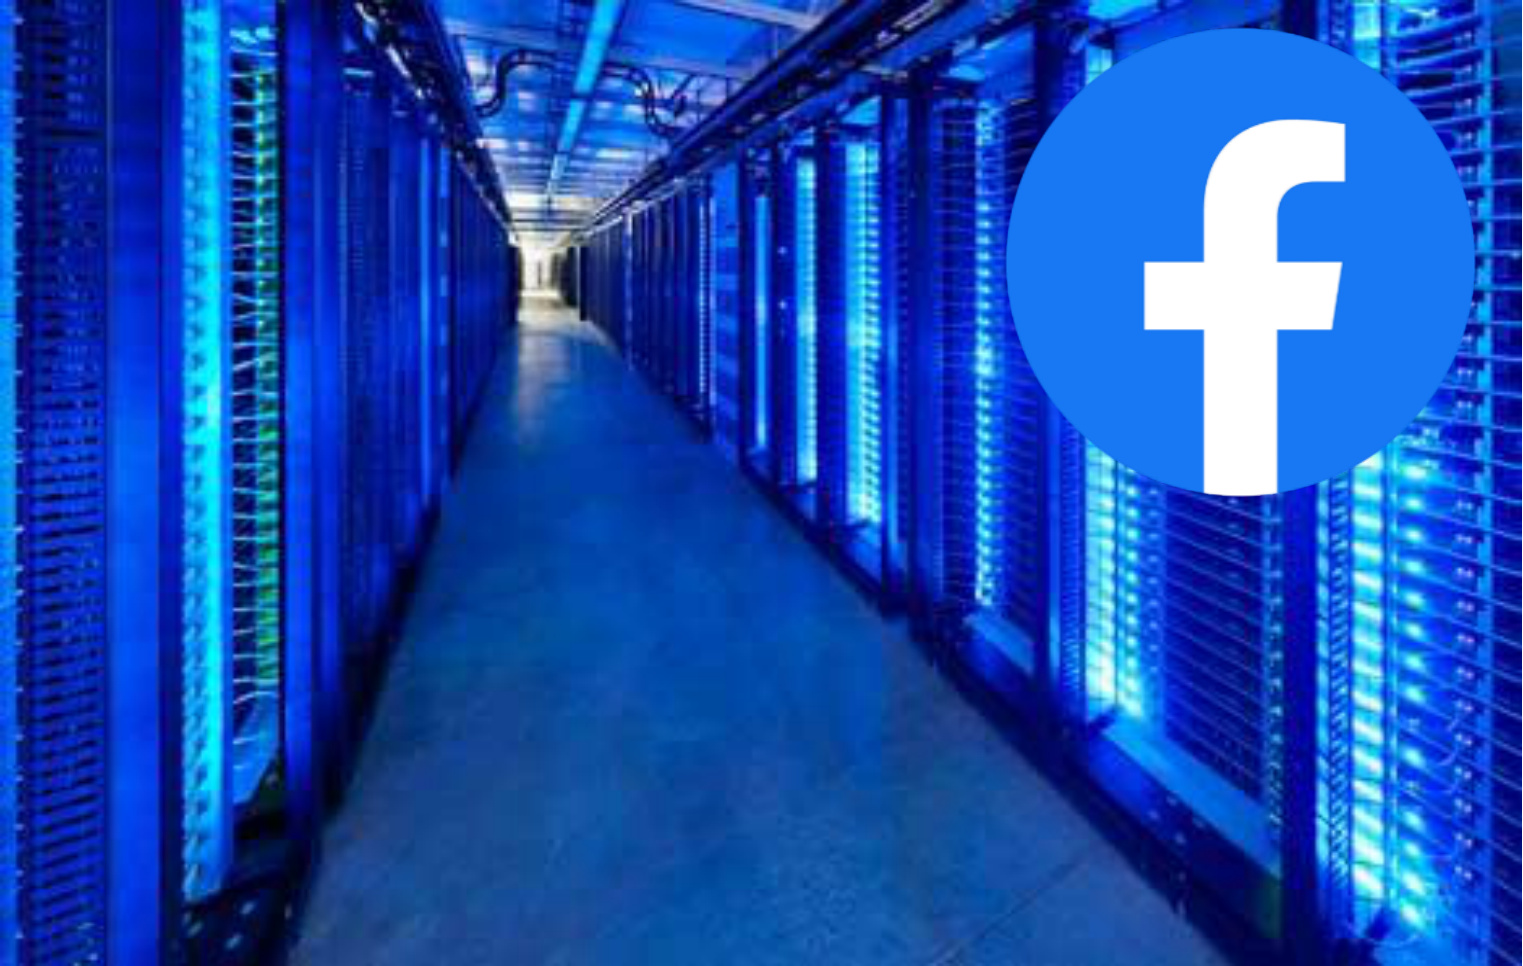
\includegraphics[width=\textwidth,height=3cm,keepaspectratio]{images/img_p21_1_128.jpeg}\\[0.15cm]
  
\includegraphics[width=0.35\textwidth]{images/img_p21_2_129.png}
\end{center}
\end{column}
\end{columns}
\end{frame}

% Slide 22: Drowning in Data - Library of Congress
\begin{frame}{ما در داده‌ها غرق شده‌ایم...}
\framesubtitle{کتابخانه کنگره آمریکا (\lr{US Library of Congress})}
\begin{columns}[T,onlytextwidth]
\begin{column}{0.55\textwidth}
\begin{itemize}
  \item \textbf{حجم محتوای متنی دیجیتال:}
  \begin{itemize}
    \item نگهداری بیش از \lr{235} ترابایت اسناد متنی آرشیوشده
  \end{itemize}
  \vspace{0.25cm}
  \item \textbf{اهداف کشف دانش و الگوها:}
  \begin{itemize}
    \item استخراج توزیع موضوعی اسناد و متون (\lr{Topic Distributions})
    \item تحلیل شبکه‌های استناد علمی (\lr{Citation Networks})
  \end{itemize}
  \vspace{0.25cm}
  \item \textbf{آموزش مدل‌های هوش مصنوعی:}
  \begin{itemize}
    \item آموزش مدل‌های زبانی بسیار بزرگ (\lr{Large Language Models})
  \end{itemize}
\end{itemize}
\end{column}
\begin{column}{0.42\textwidth}
\begin{center}
  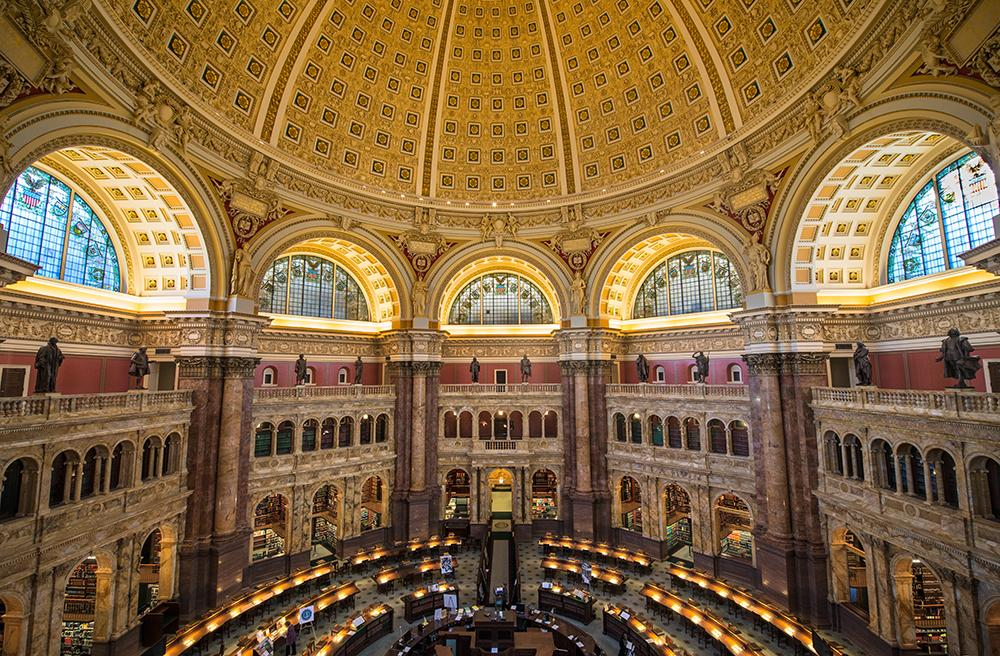
\includegraphics[width=\textwidth,height=4cm,keepaspectratio]{images/img_p22_1_135.jpeg}
\end{center}
\end{column}
\end{columns}
\end{frame}

% Slide 23: Drowning in Data - Domo
\begin{frame}{ما در داده‌ها غرق شده‌ایم...}
\framesubtitle{داده‌ها هرگز نمی‌خوابند (\lr{Data Never Sleeps 12})}
\begin{center}
  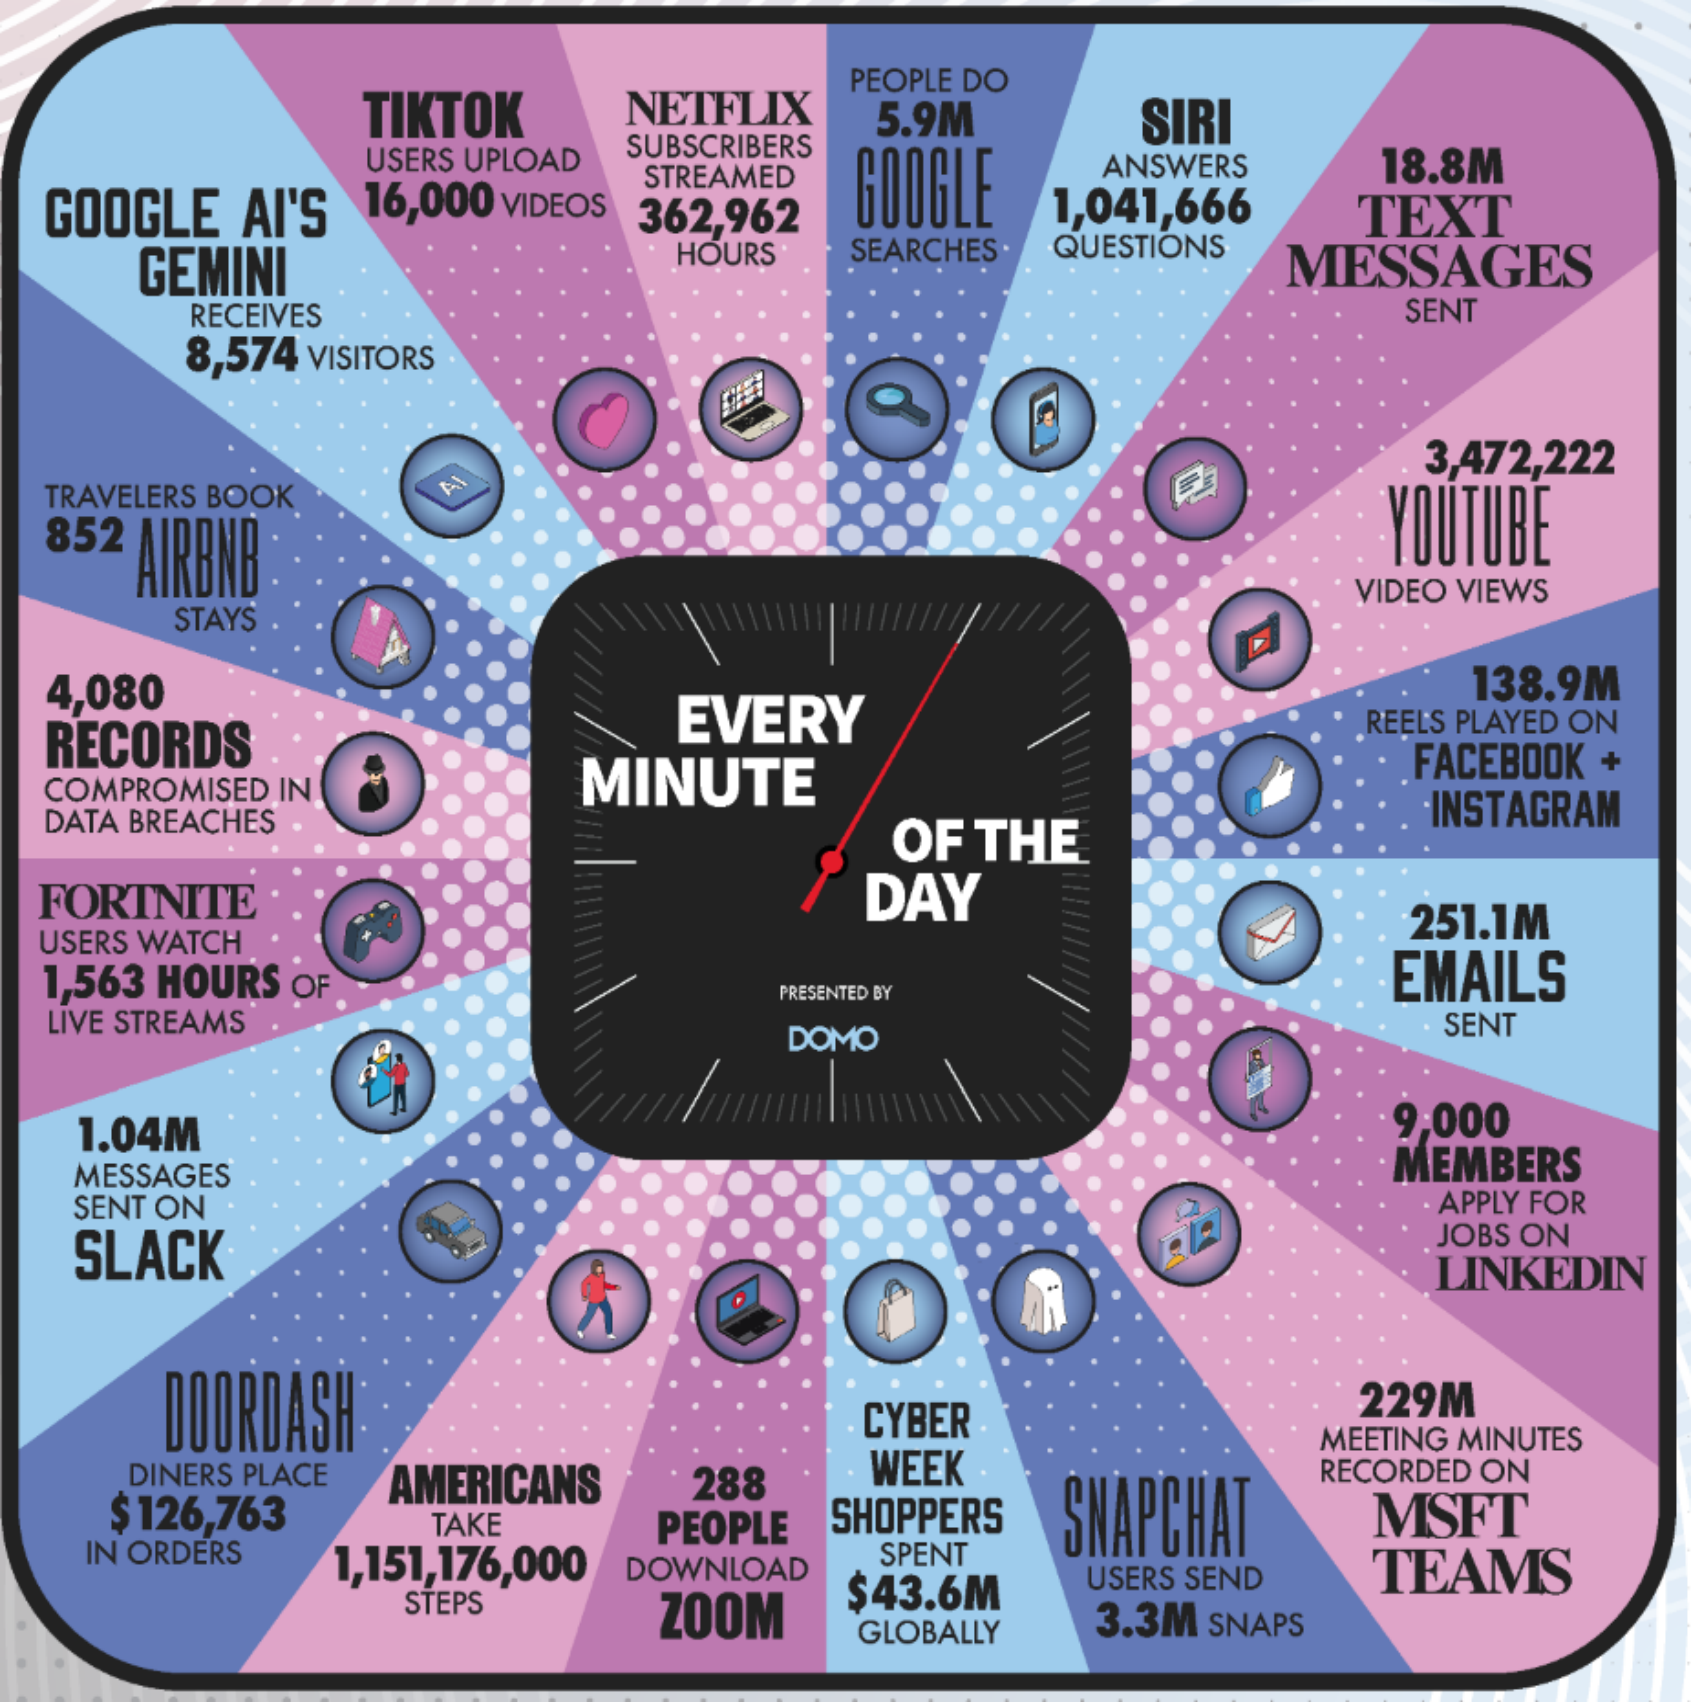
\includegraphics[width=0.72\textwidth,height=4.6cm,keepaspectratio]{images/img_p23_1_139.png}\\[0.1cm]
  {\fontsize{6.8}{8}\selectfont\color{subgray}حجم تبادل اطلاعات در هر دقیقه از اینترنت (گزارش دوازدهم شرکت \lr{Domo})}
\end{center}
\end{frame}

% Slide 24: Starving for Knowledge
\begin{frame}{غرق در داده‌ها... اما تشنه دانش!}
\begin{LTR}
\begin{columns}[c,onlytextwidth]
\begin{column}{0.38\textwidth}
\begin{center}
  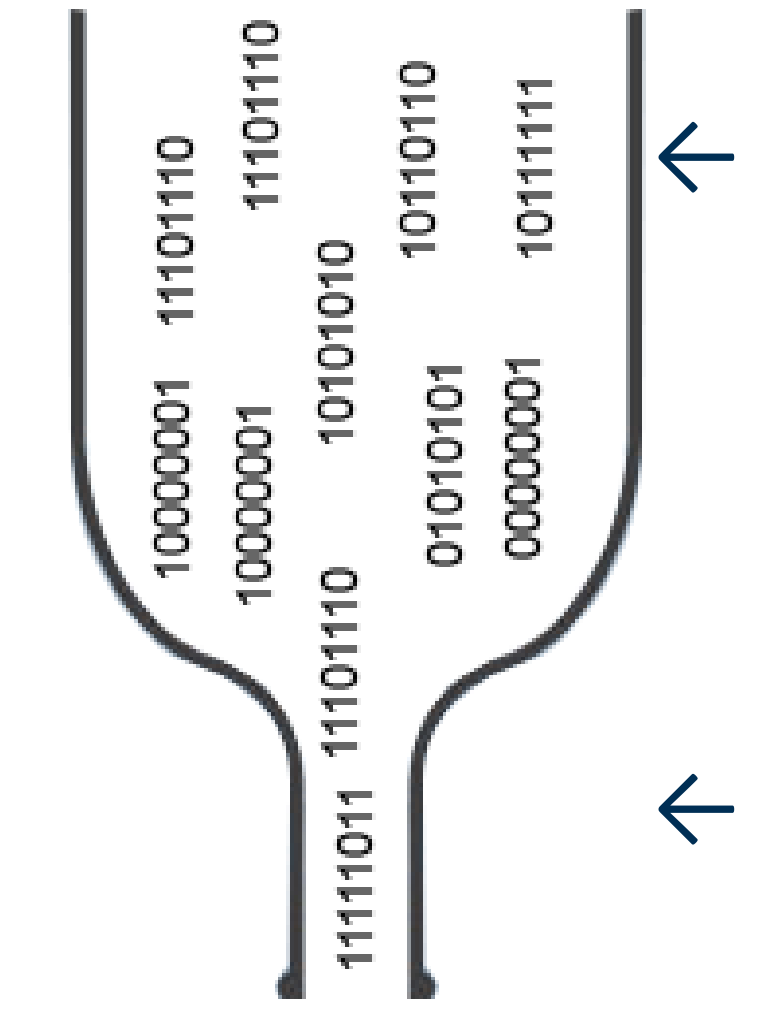
\includegraphics[width=0.85\textwidth,height=2.8cm,keepaspectratio]{images/img_p24_1_142.png}
\end{center}
\end{column}
\begin{column}{0.6\textwidth}
\raggedright
$\leftarrow$ \rl{\textbf{نرخ سرسام‌آور تولید داده‌ها}}\\[0.8cm]
$\leftarrow$ \rl{\textbf{نرخ ادراک و درک داده‌ها توسط انسان}}\\[0.15cm]
\hspace*{0.4cm}{\small\color{crimsonred}\rl{\textbf{تفسیر دستی داده‌ها عملاً غیرممکن است!}}}
\end{column}
\end{columns}
\end{LTR}
\vspace{0.25cm}
\begin{itemize}
  \item \textbf{ما به دنبال کشف الگوها هستیم، نه صرفاً انباشت داده‌های خام!}
  \item \textbf{روش‌های داده‌کاوی به ما کمک می‌کنند تا:}
  \begin{itemize}
    \item الگوهای جذاب و معنادار را در حجم انبوه داده‌ها کشف کنیم
    \item بر پایه این الگوها تصمیم‌گیری‌های دقیق و هوشمندانه اتخاذ نماییم
  \end{itemize}
\end{itemize}
\end{frame}

% Slide 25: DIKW Pyramid
\begin{frame}{هرم تبدیل داده به حکمت (\lr{DIKW})}
\begin{center}
  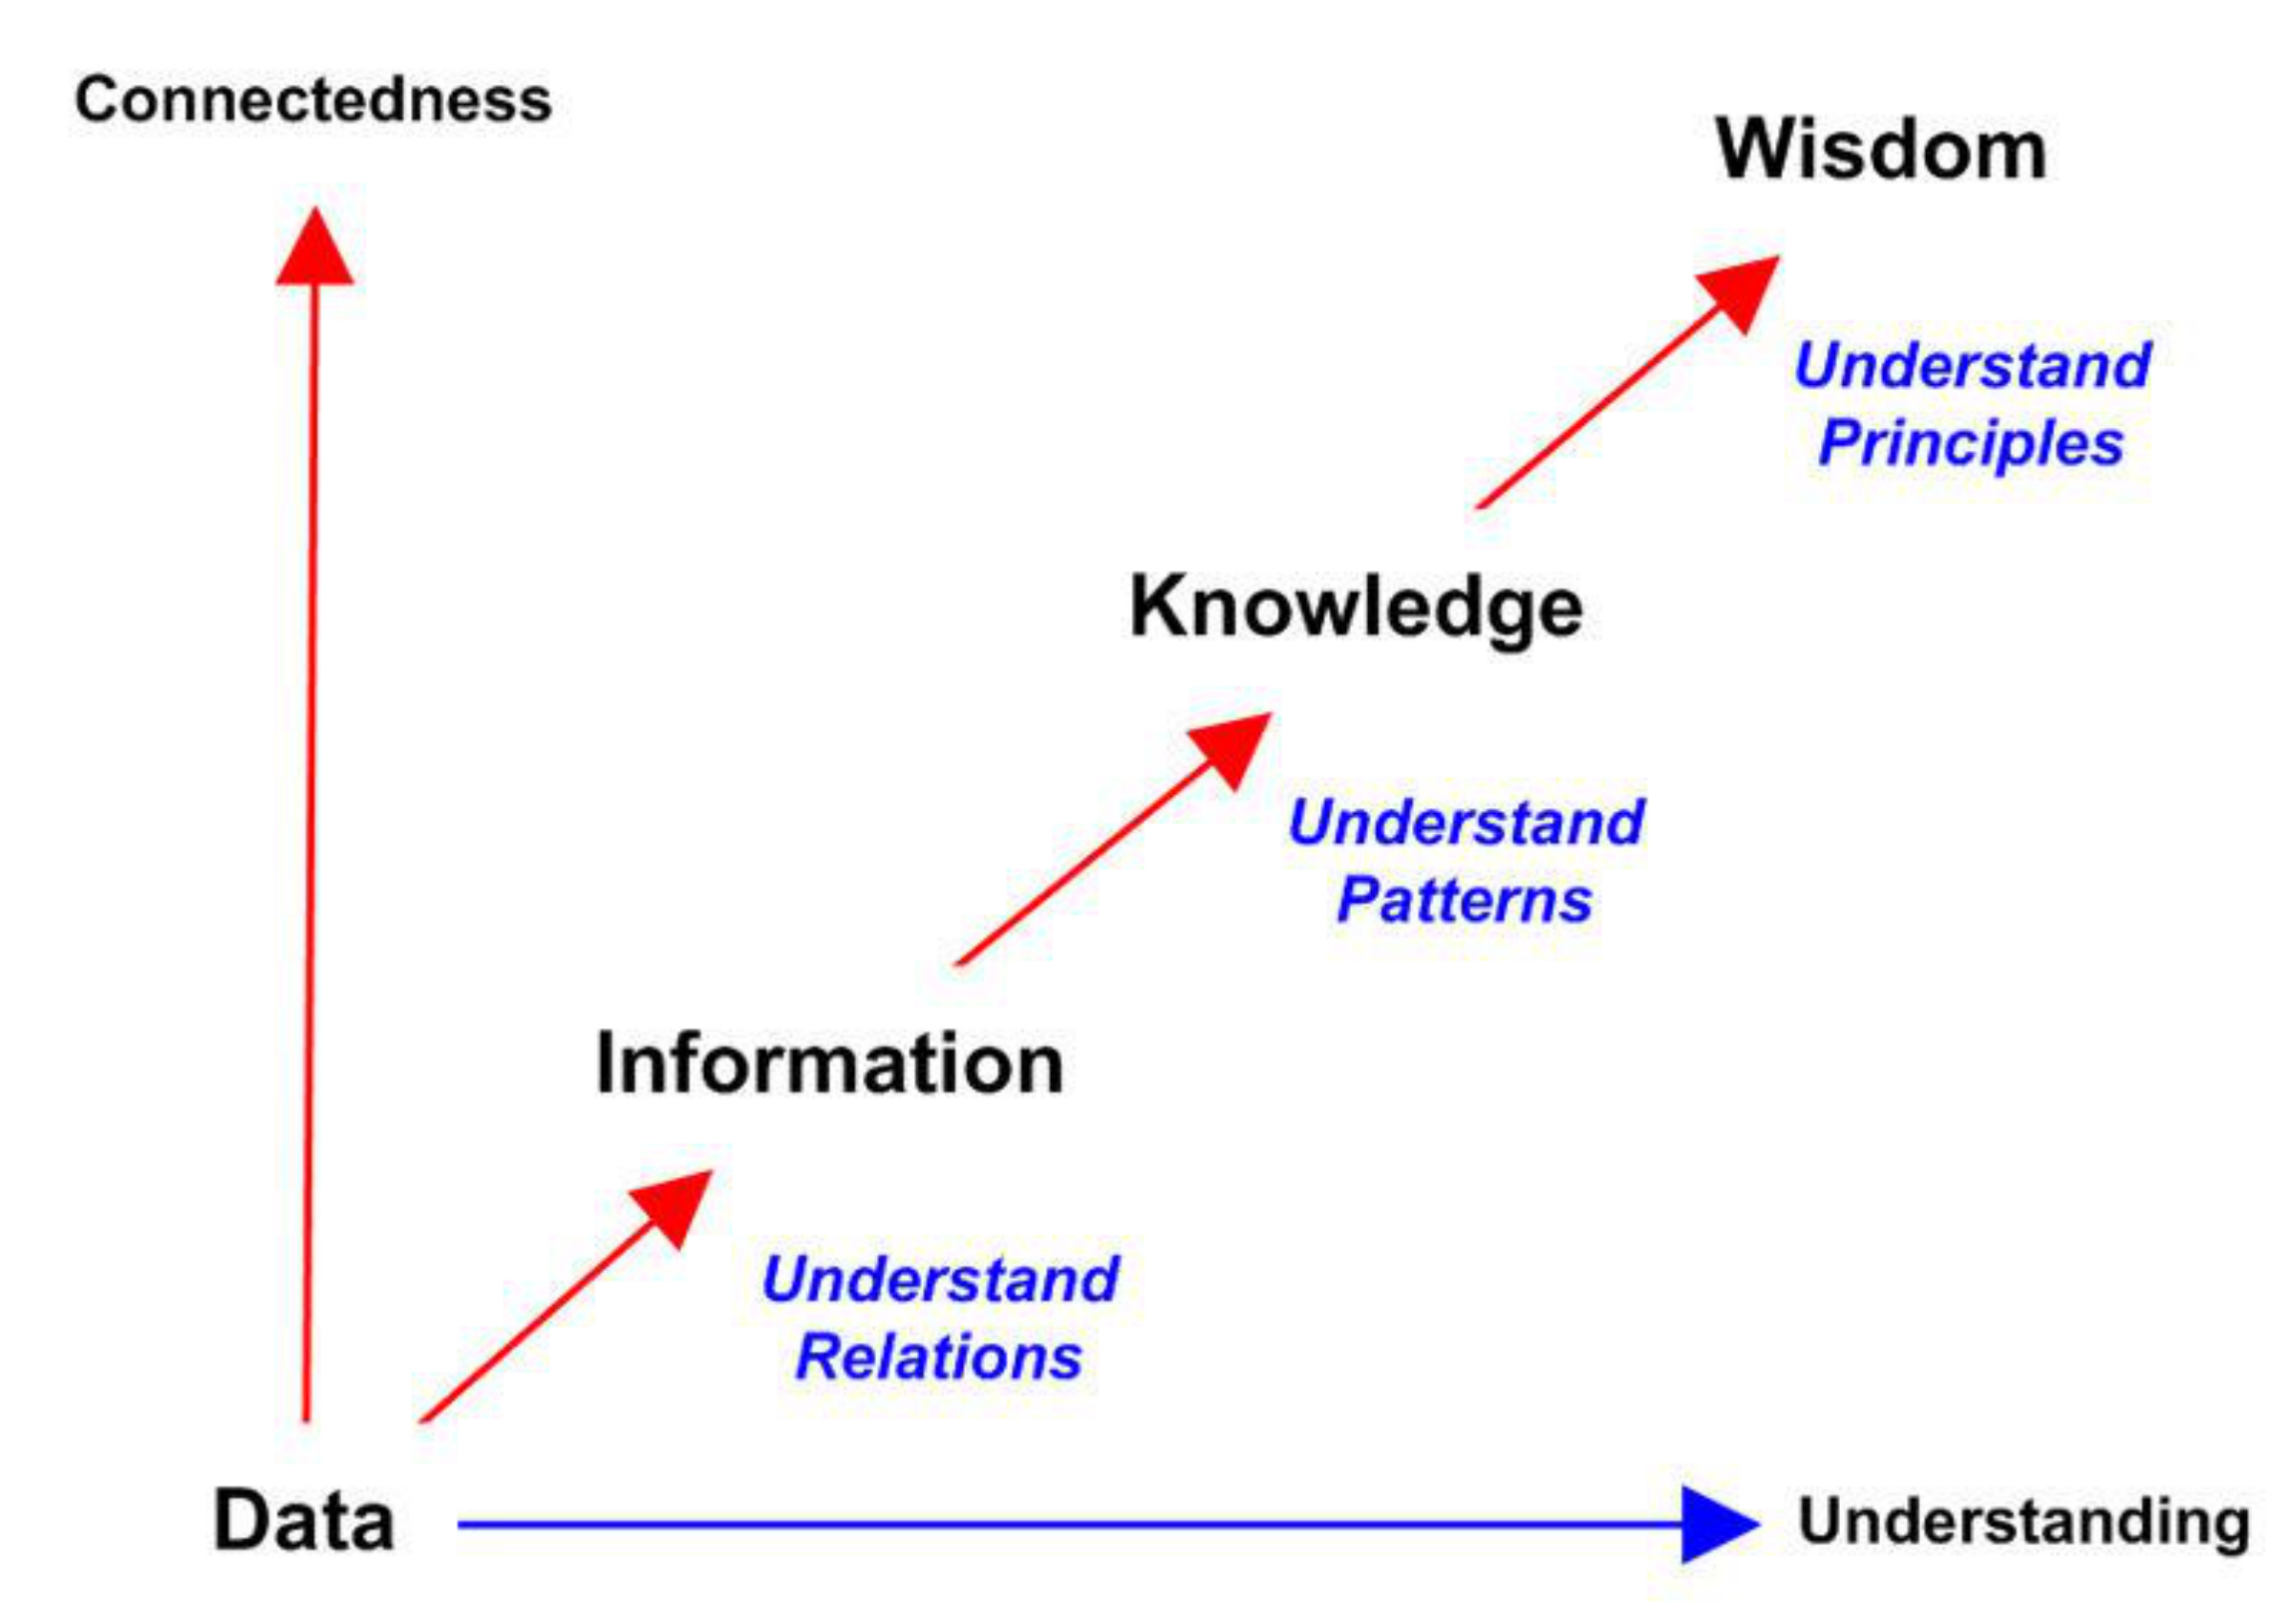
\includegraphics[width=0.88\textwidth,height=4.4cm,keepaspectratio]{images/img_p25_1_145.jpeg}\\[0.15cm]
  {\fontsize{7}{9}\selectfont\color{subgray}منبع: بلینجر، کاسترو و میلز -- سلسله‌مراتب داده (\lr{Data})، اطلاعات (\lr{Information})، دانش (\lr{Knowledge}) و حکمت (\lr{Wisdom})}
\end{center}
\end{frame}

% Slide 26: Data Mining Definitions - Analogy
\begin{frame}{تعریف داده‌کاوی -- تمثیل استخراج طلا}
\begin{itemize}
  \item \textbf{ایده بنیادین: کوه‌هایی از داده}
  \begin{itemize}
    \item مشابه کاوش در معادن برای کشف رگه‌های ارزشمند طلا از دل تن‌ها خاک و سنگ
    \item داده‌کاوی به معنای جستجو و استخراج دانش ارزشمند از دل کوه‌های عظیم داده است
  \end{itemize}
\end{itemize}
\begin{center}
  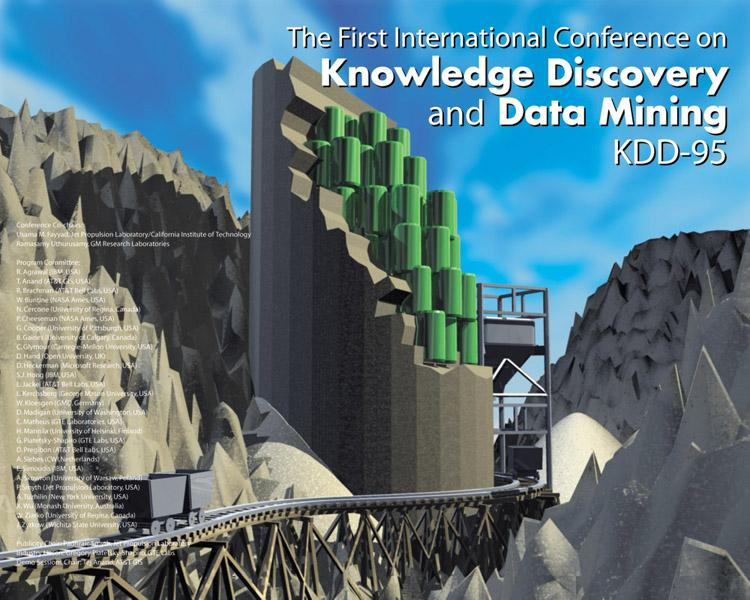
\includegraphics[width=0.62\textwidth,height=3.6cm,keepaspectratio]{images/img_p26_1_148.jpeg}
\end{center}
\end{frame}

% Slide 27: Data Mining Definitions - Fayyad
\begin{frame}{تعریف رسمی داده‌کاوی}
\framesubtitle{\lr{Fayyad et al., 1996}}
\begin{itemize}
  \item \textbf{تعریف رسمی فیاض و همکاران} (\lr{1996})
  \begin{tcolorbox}[colback=codebg,colframe=mannheimblue,arc=2mm]
    «داده‌کاوی فرآیندی \textbf{غیربدیهی} (\lr{non-trivial}) برای شناسایی الگوهای \textbf{معتبر} (\lr{valid})، \textbf{بدیع و نوظهور} (\lr{novel})، \textbf{بالقوه سودمند} (\lr{potentially useful}) و در نهایت \textbf{قابل‌فهم} (\lr{ultimately understandable}) در داده‌ها است.»
  \end{tcolorbox}
  \vspace{0.2cm}
  \item \textbf{اهداف سه‌گانه روش‌های داده‌کاوی:}
  \begin{enumerate}
    \item \textbf{کشف الگوها:} شناسایی الگوهای جذاب در مقادیر انبوه داده‌ها
    \item \textbf{پشتیبانی از تصمیم:} کمک به تصمیم‌گیری انسان با عرضه این الگوها
    \item \textbf{پیش‌بینی:} تخمین نتیجه یک مشاهده آینده بر مبنای الگوهای کشف‌شده
  \end{enumerate}
\end{itemize}
\end{frame}

% Slide 28: Origins of Data Mining
\begin{frame}{خاستگاه و علوم شکل‌دهنده داده‌کاوی}
\begin{columns}[T,onlytextwidth]
\begin{column}{0.55\textwidth}
\begin{itemize}
  \item \textbf{ترکیبی هم‌افزا از چند شاخه علمی:}
  \begin{itemize}
    \item آمار و احتمالات (\lr{Statistics})
    \item یادگیری ماشین و هوش مصنوعی (\lr{Machine Learning, AI})
    \item سامانه‌های مدیریت پایگاه‌داده (\lr{Database Systems})
  \end{itemize}
  \vspace{0.2cm}
  \item \textbf{چرا روش‌های سنتی آماری پاسخگو نیستند؟}
  \begin{itemize}
    \item حجم بسیار عظیم داده‌ها (\lr{Large amount of data})
    \item ابعاد بالا و متغیرهای متعدد (\lr{High dimensionality})
    \item ماهیت ناهمگون و توزیع‌شده داده‌ها (\lr{Heterogeneous, distributed})
  \end{itemize}
\end{itemize}
\end{column}
\begin{column}{0.43\textwidth}
\begin{center}
  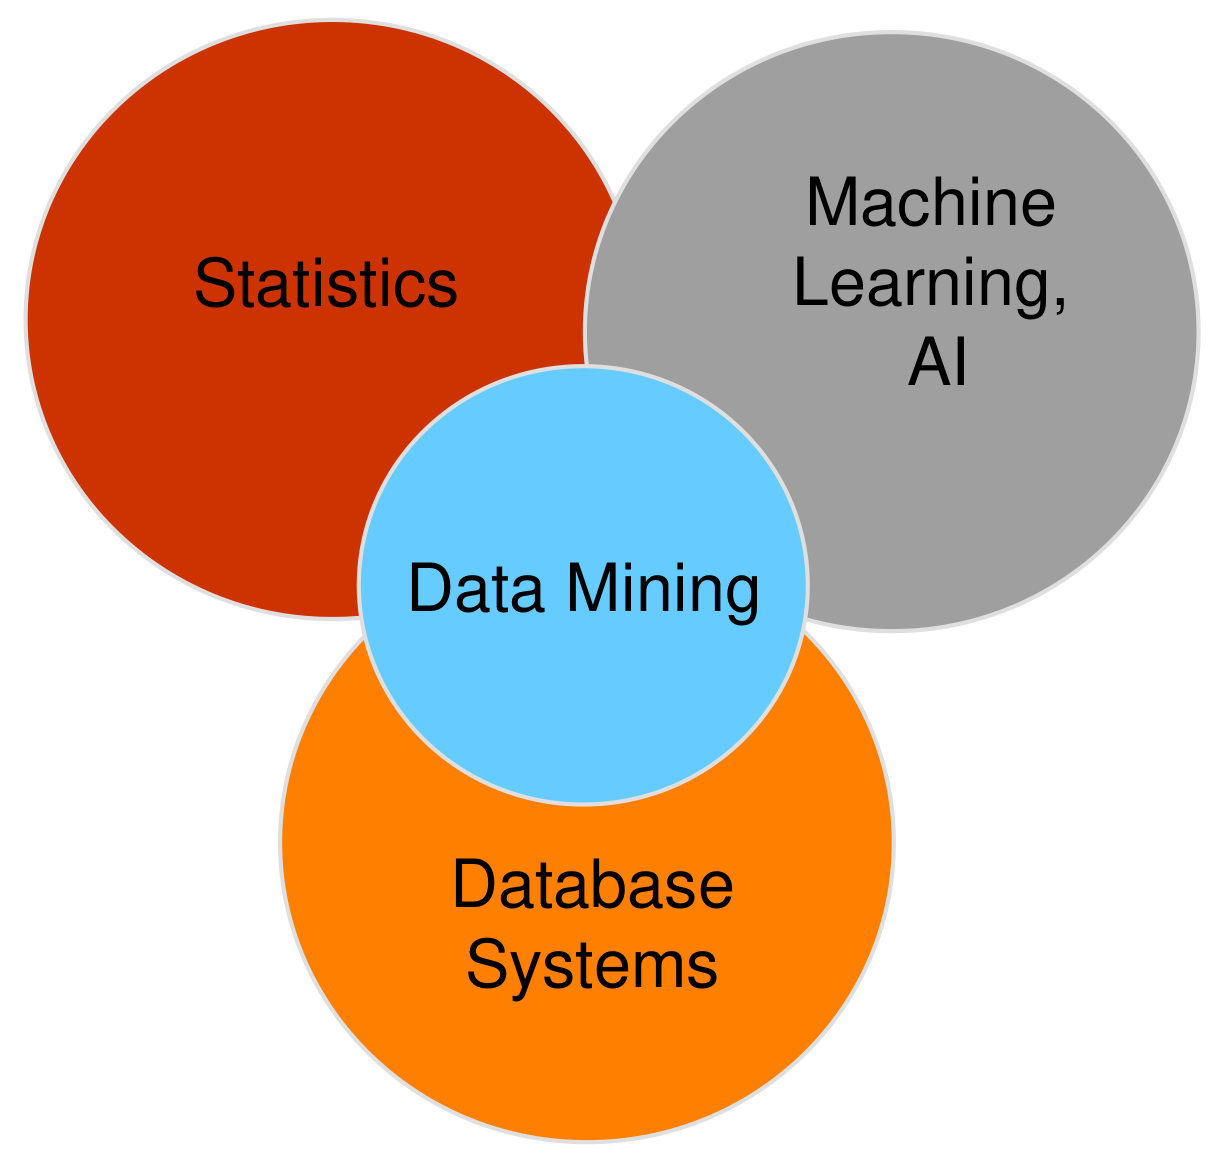
\includegraphics[width=\textwidth,height=4.2cm,keepaspectratio]{images/diagram_p28_origins_venn.png}
\end{center}
\end{column}
\end{columns}
\end{frame}
